\subsection{KNN}
En esta sección definimos:
\begin{itemize}
	\item $k$: cantidad de vecinos a considerar en el algoritmo $kNN$.
\end{itemize}
El análisis sobre el algoritmo $KNN$ ($k$ vecinos más cercanos) se realiza para distintos valores de $k$, la idea detrás de esto es comprender la variación en la efectividad (cantidad de aciertos) del algoritmo a través del ajust de este parámetro.
\\
Para ello variamos $k$ desde $1$ hasta $30$ para ver cual es su comportamiento. Para cada uno de los $k$ vecinos realizamos una corrida de cross-validation con $10$ conjuntos.
\\
% El procedimiento de este algoritmo comienza, por cada imágen que queremos averiguar a que dígito pertenece, con su vectorización. Luego resta el resultado a cada uno de los vectores imágen y calcula la norma 2 para saber en cuánto difieren con cada una de las imágenes.
% Todos esos resultados se acumulan en una cola de prioridad que los ordena de menor a mayor, según las diferencias entre la imágen la cual se quiere averiguar a que clase pertenece y todas las imágenes de la base de datos etiquetada.
% \\
% Como siguiente paso se toman los $k$ primeros elementos de la cola de prioridad y se verifica a que dígito se corresponden para luego saber cuál es el dígito que recibió más "votos" y ver si se produjo un acierto o no.
% \subsubsection{Cantidad de vecinos}
% Como ya dijimos, para analizar cuál es el mejor número de vecinos para el cual el algoritmo $KNN$  da una mayor cantidad de aciertos, optamos por variar la cantidad de $k$ vecinos a tomar.
%Se prueba entonces el algoritmo $KNN$ para los siguientes valores de $k$: $1,2,3,4,...,30$.
%\\
Cada uno de los conjuntos contó con 4200 imágenes a testear. En los siguientes gráficos presentamos algunos de los sets obtenidos:
\begin{center}
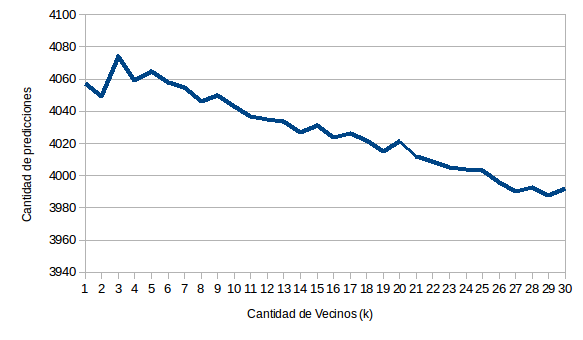
\includegraphics[scale=0.55]{nuevosResultados/knn/1.png}
\end{center}

\begin{center}
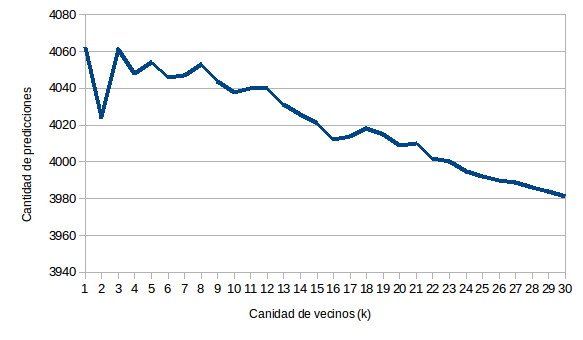
\includegraphics[scale=0.55]{nuevosResultados/knn/2.png}
\end{center}

\begin{center}
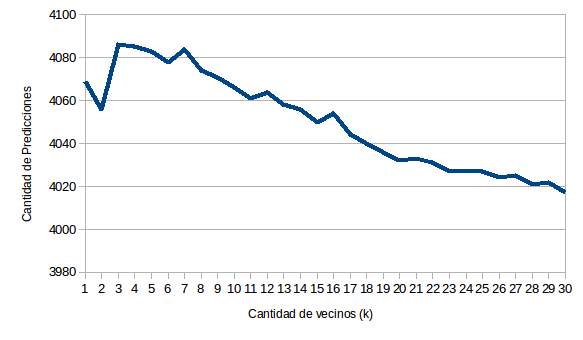
\includegraphics[scale=0.55]{nuevosResultados/knn/3.png}
\end{center}
\begin{center}
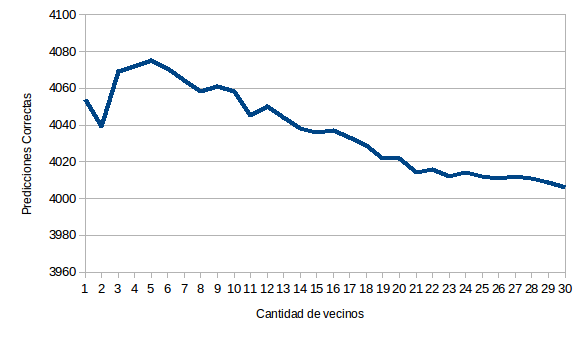
\includegraphics[scale=0.55]{nuevosResultados/knn/4.png}
\end{center}


Como se puede ver hay un patrón bastante claro en los experimentos realizados, para valores muy pequeños de $k$ los resultados son bastante buenos. Para $k=1$ se obtiene el mejor valor para $3$ de los sets que testeamos, para $k=3$ se obtiene que $4$ veces es la cantidad de vecinos que produce más aciertos, para el resto de los sets se encuentran también valores cercanos a estos. Para valores más grandes se observa un comportamiento que ratifica nuestra intuición, con un gran número de vecinos se empiezan a perder aquellos que son realmente relevantes y las predicciones empiezan a ser peores. Lo que no se esperaba era el salto en la cantidad de aciertos que vemos en los primeros valores de $k$ pero podemos entonces saber que dentro de los primeros $k$ se encuentran los mejores resultados.
\\
La distribución del mejor $k$ es la siguiente:
\begin{center}
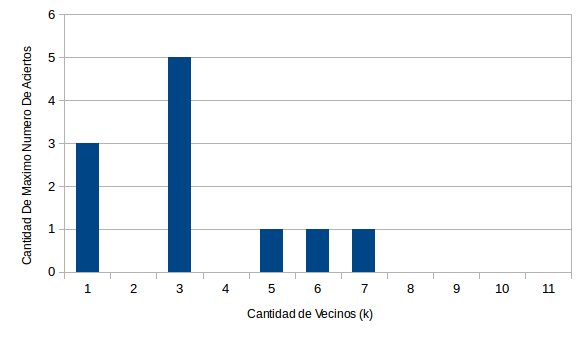
\includegraphics[scale=0.55]{nuevosResultados/knn/max.png}
\end{center}
Decidimos luego que el mejor valor para $k$ es el que produce más veces el máximo número de aciertos, es decir $k=3$. La conclusión que podemos extraer de este resultado es que para ciertos casos puede pasar que la imagen que está en primer lugar de la cola de prioridad no sea la correcta, eso pasaría para el caso en que se tiene un dígito que se parece mucho al primero de la cola, pero estos no son iguales.
Por ejemplo teniendo el dígito $x$, testeandolo con una base de datos grande en la que ningún dígito $x'$ se parece a $x$, pero teniendo otro dígito $y$ tal que se parece mucho, ese dígito $y$ va a quedar en la primera posición de la cola de resultados.
Recordemos que una vez que comparamos el dígito con toda la base de datos, se arma una cola de prioridad, ordenados semejanza entre dígitos.
Como decíamos, ese dígito $y$ puede ser considerado como un 'outlier', ya que hace que el dígito más parecido no sea el resultado correcto. Por lo tanto siempre es mejor elegir más vecinos para saber cuales dígitos aparecen en mayor cantidad y así seleccionar el de mayor cantidad de apariciones.
\\ \\
Pero, ¿Hasta qué cantidad de vecinos conviene tomar?
Si elegimos pocos vecinos podríamos tener el problema comentado anteriormente de elegir el dígito más cercano pero no el correcto.
Si elegimos muchos vecinos, lo que podría pasar es que estaríamos contando los dígitos que menos se parecen al dígito testeado, o sea, estaríamos eligiendo los peores resultados.
Según los resultados obtenidos, nos conviene elegir los primeros 3 vecinos más cercanos, ya que según los resultados testeados es el que más cantidad de aciertos obtuvo.
\\ \\
Otra observación que podemos ver de las imágenes resultantes es que para los valores $k$ pares obtenemos una menor cantidad de aciertos que para los $k$ impares.
Esto tiene sentido, ya que si tengo un dígito $x$ a testear y en la cola de prioridad obtengo como los dígitos más cercanos, por ejemplo, los dígitos $x$, $y$, $x$, $y$.
Si elegimos $k=1$ o $k=3$ el resultado sería correcto, pero si elegimos un valor $k$ par, podríamos tener un empate entre 2 dígitos y podríamos elegir el dígito incorrecto simplemente al azar, por una elección arbitraria del algoritmo, o por cualquier motivo para desempatar. Entonces por ese simple motivo, podríamos elegir mal el dígito correcto y tener menor cantidad de aciertos. En cambio, para los $k$ impares ese problema no lo tenemos y nos evitaríamos ese inconveniente, por más que después se elija el resultado correcto o no.
\\ \\
Además para estos tests realizamos una medición de tiempos para ver cómo se comportaba el algoritmo frente a un cambio en la cantidad de vecinos. Los valores promediados para cada $k$ pueden verse en el siguiente gráfico:

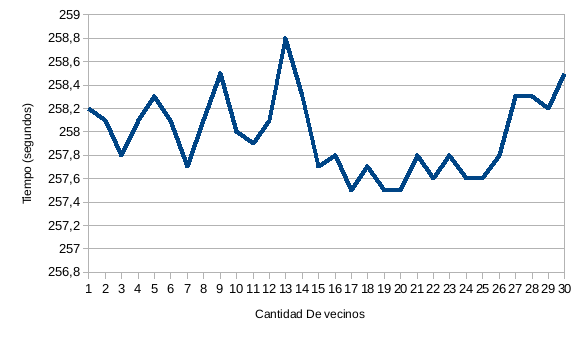
\includegraphics[scale=0.55]{nuevosResultados/knn/knntemp.png}\\

Como puede observarse, los tiempos de los algoritmos no se ven muy afectados por la variación en la cantidad de vecinos. Es muy probable que esto se deba a que el algoritmo debe comparar a la imagen que se desea comparar contra un número muy extenso de imágenes que estan en el mismo orden de magnitud.
%completar

Luego de los test decidimos que vamos a usar $k=3$ porque nos dio los mejores resultados, basado en la  cantidad de aciertos.

\subsection{PCA}
\subsubsection{Búsqueda del mejor valor de $\alpha$}
En esta sección definimos:
\begin{itemize}
	\item $\alpha$: a la cantidad de componentes principales a tomar para el $PCA$.
	\item $k$: cantidad de vecinos a considerar en el algoritmo $kNN$.
\end{itemize}
En primera instancia vamos a utilizar el método de cross-validation para intentar determinar el mejor $\alpha$ posible. Supondremos en este momento que el mejor $k$ para este caso es el encontrado en la sección anterior (aunque esto podría no ser así) y luego testeamos si esto es así o si para el $\alpha$ encontrado existe algun otro $k$ que mejora la cantidad de predicciones del sistema.
\\
Por lo tanto enfocamos nuestro análisis en obtener un valor óptimo de $\alpha$. Para este fin, partimos el conjunto de datos de entrenamiento en 10 subconjuntos y aplicamos cross-validation. Dado que este parámetro representa la cantidad de componentes principales a tener en cuenta y teniendo en mente el funcionamiento del algoritmo de $PCA$, es esperable que valores pequeños no sean beneficiosos (teniendo en cuenta que el máximo a considerar es bastante elevado), pero dado que el método de $PCA$ las ordena en base a su relevancia, se alcance un valor óptimo sin necesidad de considerarlas todas. Para esta partición de los datos de entrenamiento con 4200 imágenes para testear, tomamos $\alpha$ desde $1$ hasta $50$ y graficamos lo obtenido:

\begin{center}
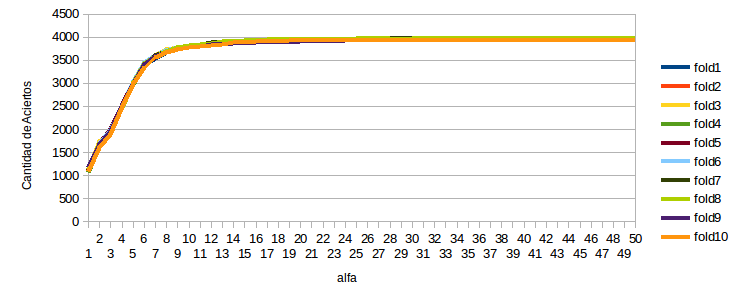
\includegraphics[scale=0.6]{nuevosResultados/pca/alfa/1.png}
\end{center}

Puede verse que para valores pequeños, aumentar en uno el $\alpha$ produce un gran aumento de aciertos. Por ejemplo, considerando el primer set para $\alpha$ igual a $1$ se obtienen $1112$ aciertos, mientras que para $\alpha$ igual a $2$ se obtienen $1680$ aciertos, esto representa un $52\%$ más de aciertos.
\\
Para valores más grandes de $\alpha$ (alrededor de $\alpha = 12$) esta tendencia empieza a estabilizarse. Por ejemplo para $\alpha = 12$ se obtienen $3845$ imágenes correctamente predecidas, pero para $\alpha = 13$ se obtienen $3869$ imágenes correctas, esto es el crecimiento de aciertos es de menos de un $1\%$.
\\
Además, para este $k-fold$ medimos los tiempos de ejecución y los promediamos para poder ver de que manera varía la ejecución de los algoritmos en función de $\alpha$:

\begin{center}
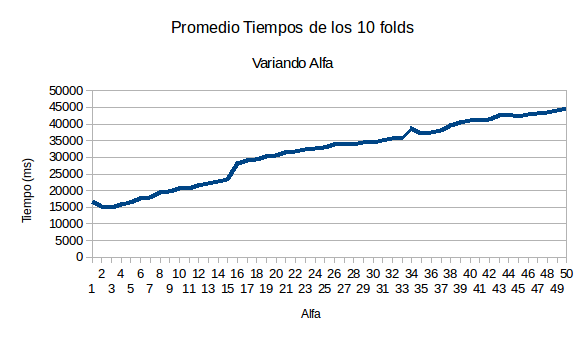
\includegraphics[scale=0.6]{nuevosResultados/pca/alfa/temp.png}
\end{center}


Cabe aclarar que estos tiempos no contemplan todo lo que se considera el 'entrenamiento' del sistema, es decir, todo el preprocesamiento que resultará en encontrar los valores principales. La justificación de esto es que el procedimiento se realizará una vez, para entrenar el sistema y luego, al momento de clasificar las nuevas imágenes este tiempo podrá ser despreciado.
\\
En este gráfico se puede ver que aumentar el $\alpha$ produce un aumento lineal de los tiempos de ejecución, de lo que se desprende que aumentar la cantidad valores principales no resulta gratuito en términos de tiempo de ejecución y tiene cierto costo asociado.
\\
Además aumentar de manera desmedida el $\alpha$ puede provocar lo que en la jerga de machine learning se denomina 'Overfitting' o Sobreajuste, que consiste en que el modelo en vez de buscar patrones sobre los cuales predecir, empieza a 'memorizar' de alguna manera los datos de entrenamiento. Esto puede conducir a que, si bien en la etapa de desarrollo se obtienen buenos niveles de predicción, cuando el modelo es puesto a prueba en algún caso real su desempeño no es el esperado\footnote{\label{note1}A Few Useful Things to Know about Machine Learning, Pedro Domingos, Department of Computer Science and Engineering, University of Washington}.
\\
Debido a todas las razones expuestas consideramos que $\alpha$ igual a $14$ será el mejor valor que podemos tomar.
\\
%falta retestear esto de abajo
\subsubsection{Búsqueda del mejor valor de $k$}

La segunda prueba a realizar es, fijando un valor de $\alpha$, analizar para que cantidad de vecinos se obtiene la mayor cantidad de aciertos.
\\
Para esto tomamos $\alpha = 14$, volvemos a dividir el conjunto de datos en $10$ sets y realizamos cross validation sobre estos, variando el $k$ desde $1$ hasta $30$.
\\
En el siguientes gráficos mostramos el resultado obtenido para los tres de los sets cuando se varía el número de vecinos:
\begin{center}
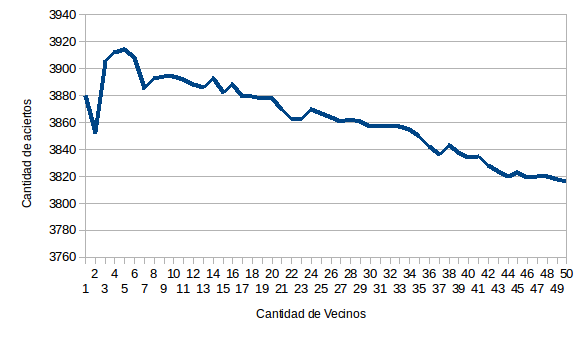
\includegraphics[scale=0.6]{nuevosResultados/pca/k/1.png}\\
\end{center}
\begin{center}
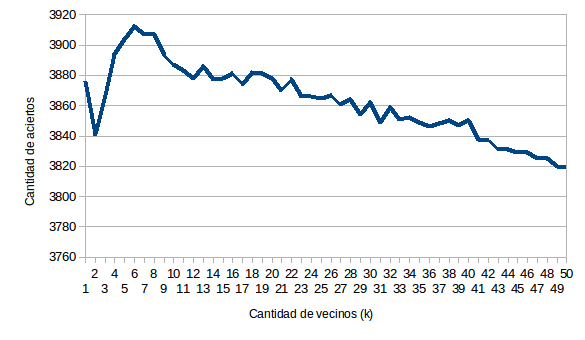
\includegraphics[scale=0.6]{nuevosResultados/pca/k/2.png}\\
\end{center}
\begin{center}
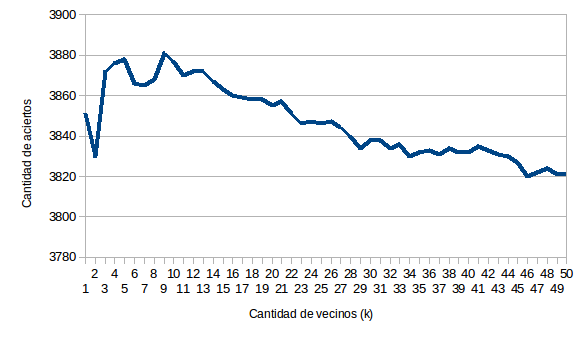
\includegraphics[scale=0.6]{nuevosResultados/pca/k/3.png}\\
\end{center}

En total, de los diez sets en tres de ellos se encontró que el número de vecinos que maximiza la cantidad de aciertos era $5$, en dos se encontró que el máximo fue $7$ y $8$, y en otros restantes el mejor fue $3$, $6$ y $9$ vecinos, cada uno.
\\
En el siguiente gráfico expresamos cómo se distribuyeron los máximos en cada conjunto del cross-validation:
\begin{center}
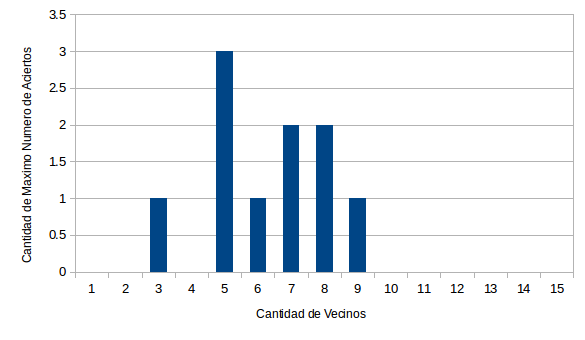
\includegraphics[scale=0.6]{nuevosResultados/pca/k/mejores.png}\\
\end{center}
De esto podemos determinar que el $k$ óptimo se encuentra en un rango entre $3$ y $9$.

Además medimos los tiempos y los promediamos para obtener una idea de cómo afectan las variaciones de $k$ a este método:
\begin{center}
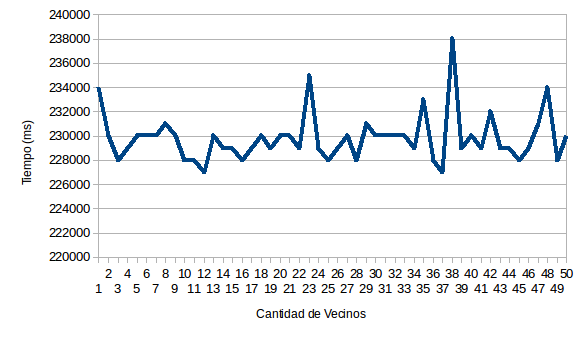
\includegraphics[scale=0.6]{nuevosResultados/pca/k/temp.png}\\
\end{center}

Como podemos ver, el número de vecinos continúa sin afectar mayormente los tiempos de ejecución incluso luego de haber reducido la dimensión de la entrada.
